\documentclass[12pt,a4paper]{article}
\usepackage{amsmath}
\usepackage[margin=2cm]{geometry}
\usepackage[ngerman]{babel}
\usepackage[utf8]{inputenc}

\usepackage{setspace}
\usepackage{xcolor}

\usepackage{siunitx}
\sisetup{locale=DE}

\usepackage{booktabs}
\usepackage{graphicx}

\usepackage{float}
\usepackage{lmodern}
\usepackage[T1]{fontenc}

\begin{document}
\setlength{\parindent}{0pt}


\title{Exercise 1, Handwritten Exercises}
\author{Dominik Autaler, Jonas Otto}

\maketitle

\section{}

\subsection{Aufgabe 2.1}
Given the image $I = \left( \begin{array}{rrrrr}0 & 0 & 1 & 1 & 1 \\0 & \color{red}0 & \color{red}1 & \color{red}0 & 0\\0 & 0 & 0 & 0 & 0\\0 & 0 & 1 & 1 & 0\\\end{array}\right) $ and the filter $G_x = \left( \begin{array}{rrr}-1 & 0 & 1\\-1 & \color{green}0 & 1\\-1 & 0 & 1\\\end{array}\right)$ the values of the three marked pixels are (from left to right) 2, 1 and -1.

\subsection{Aufgabe 2.2}
\begin{figure}[h]
	\begin{center}
		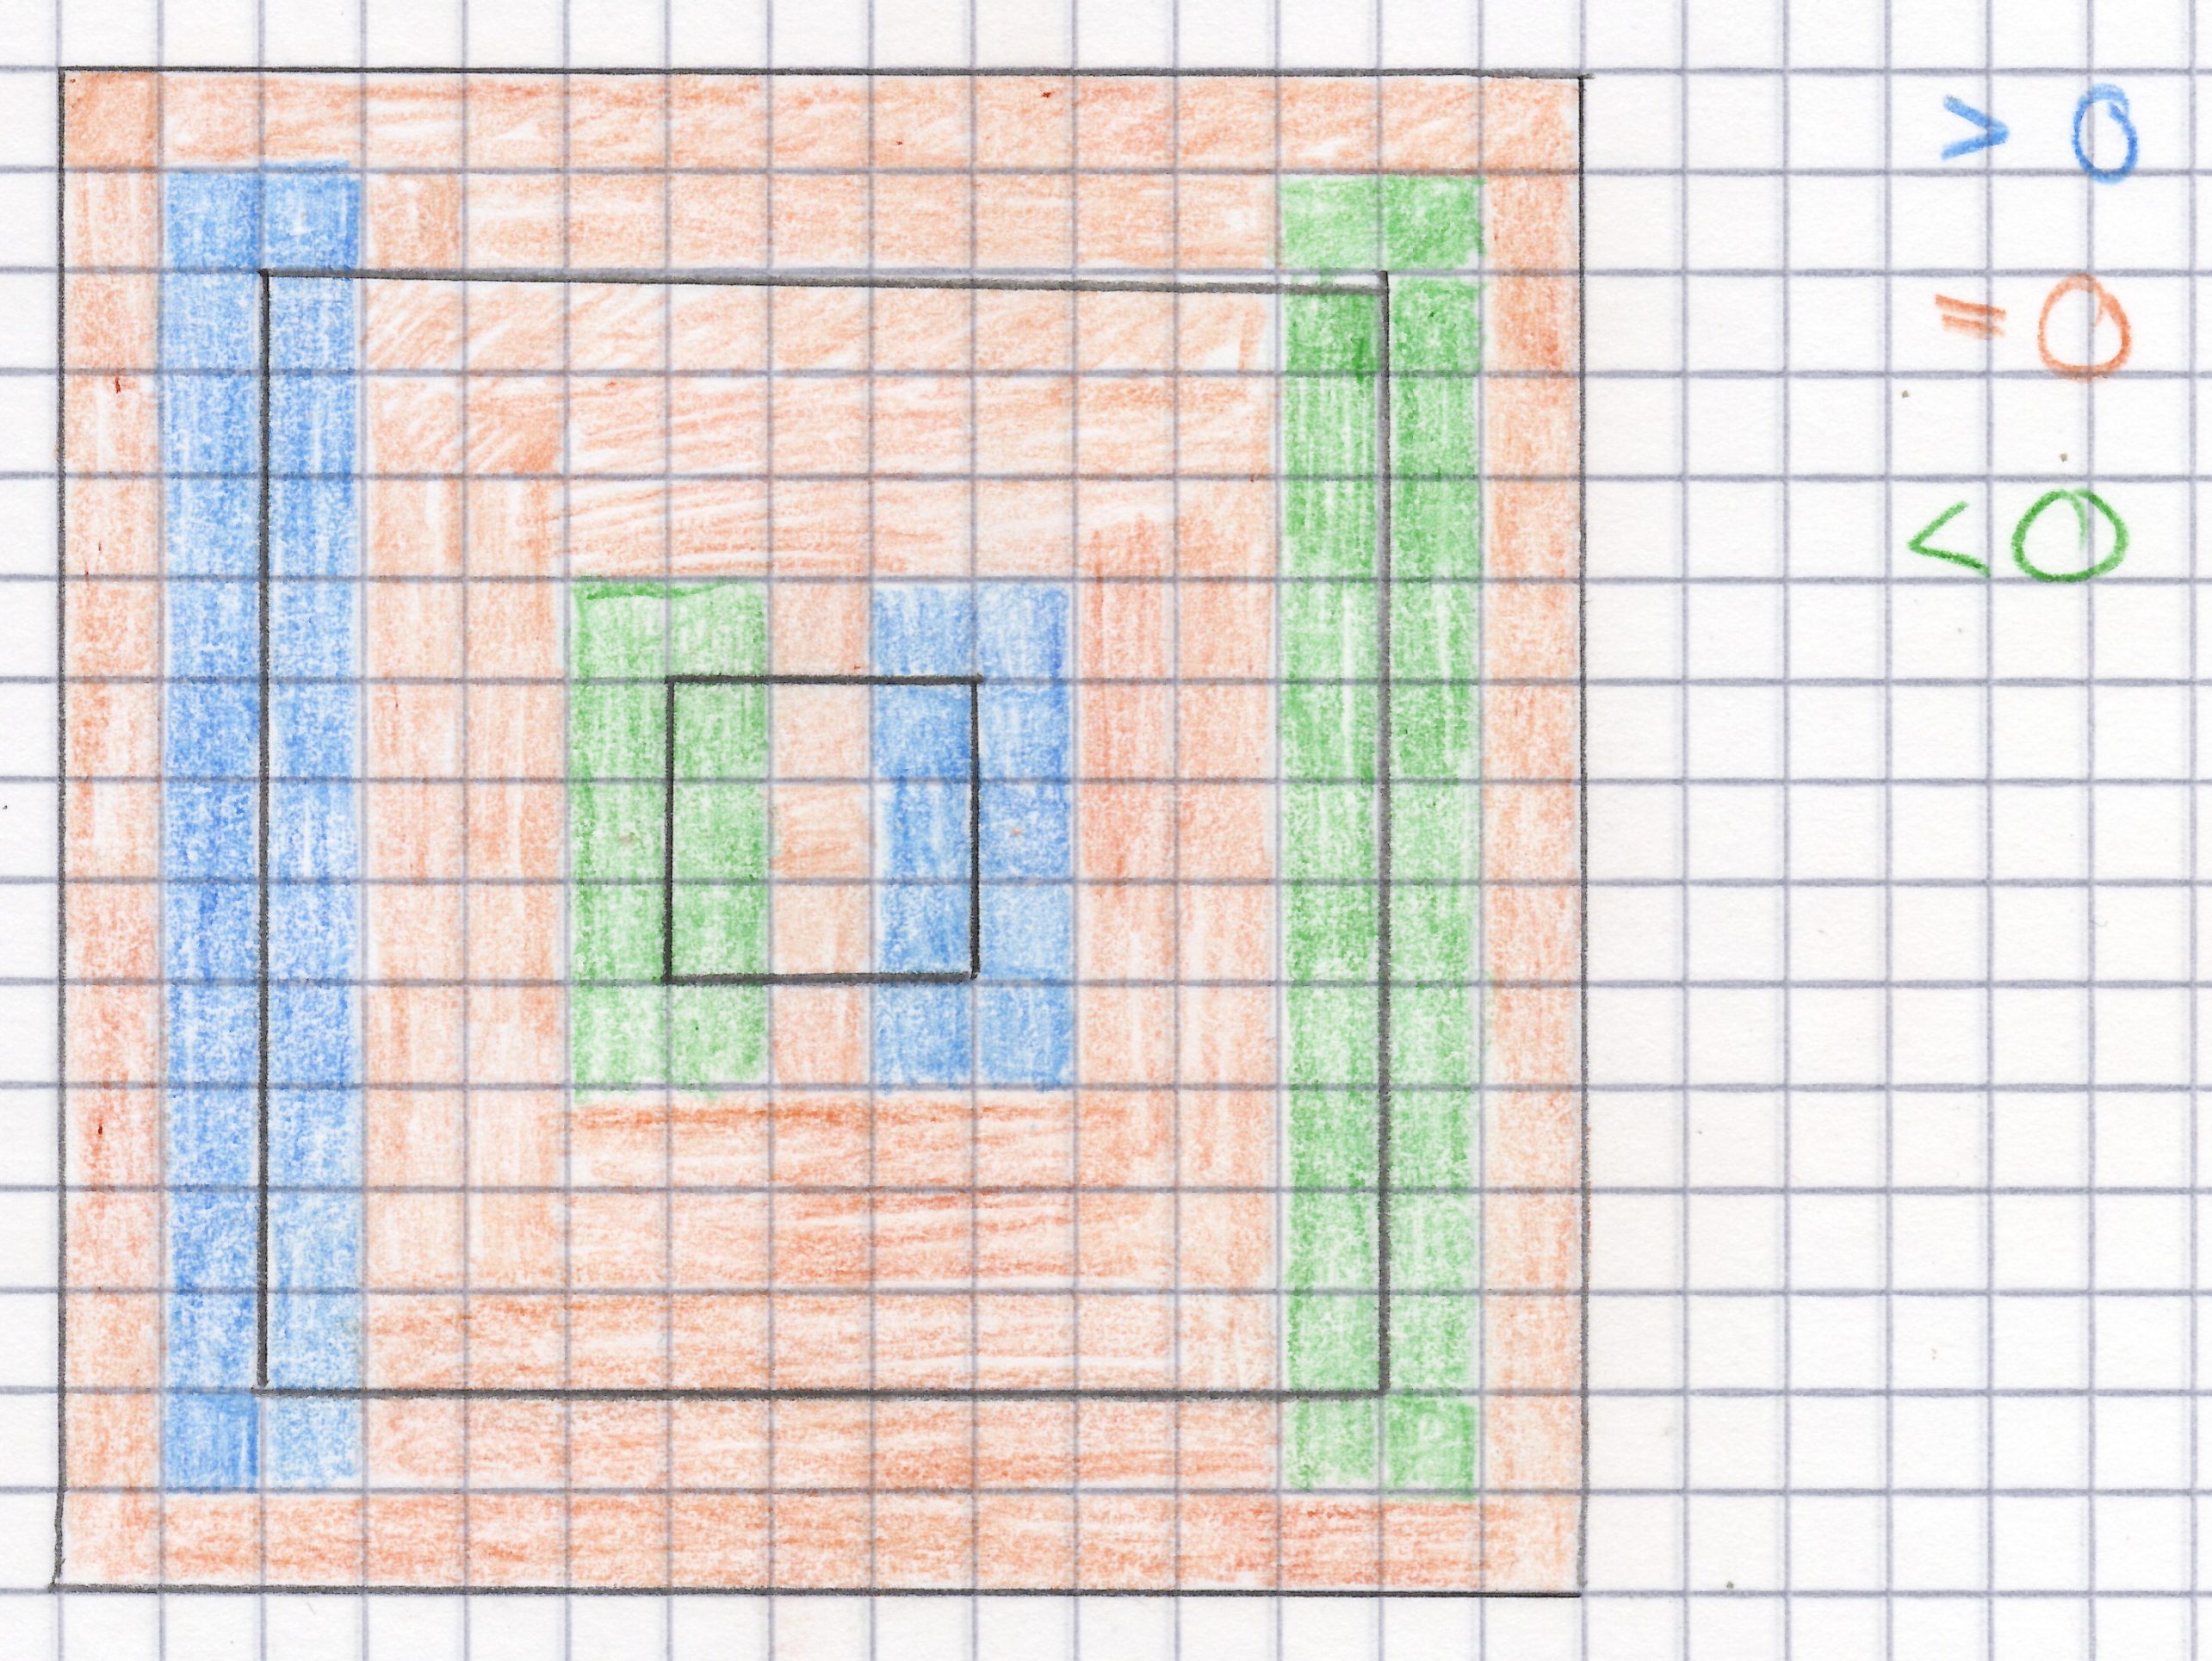
\includegraphics[scale=0.25]{GX.png}
		\caption{Response type of $G_x$ applied to the Figure} 
	\end{center}
\end{figure}

\begin{figure}[h]
	\begin{center}
		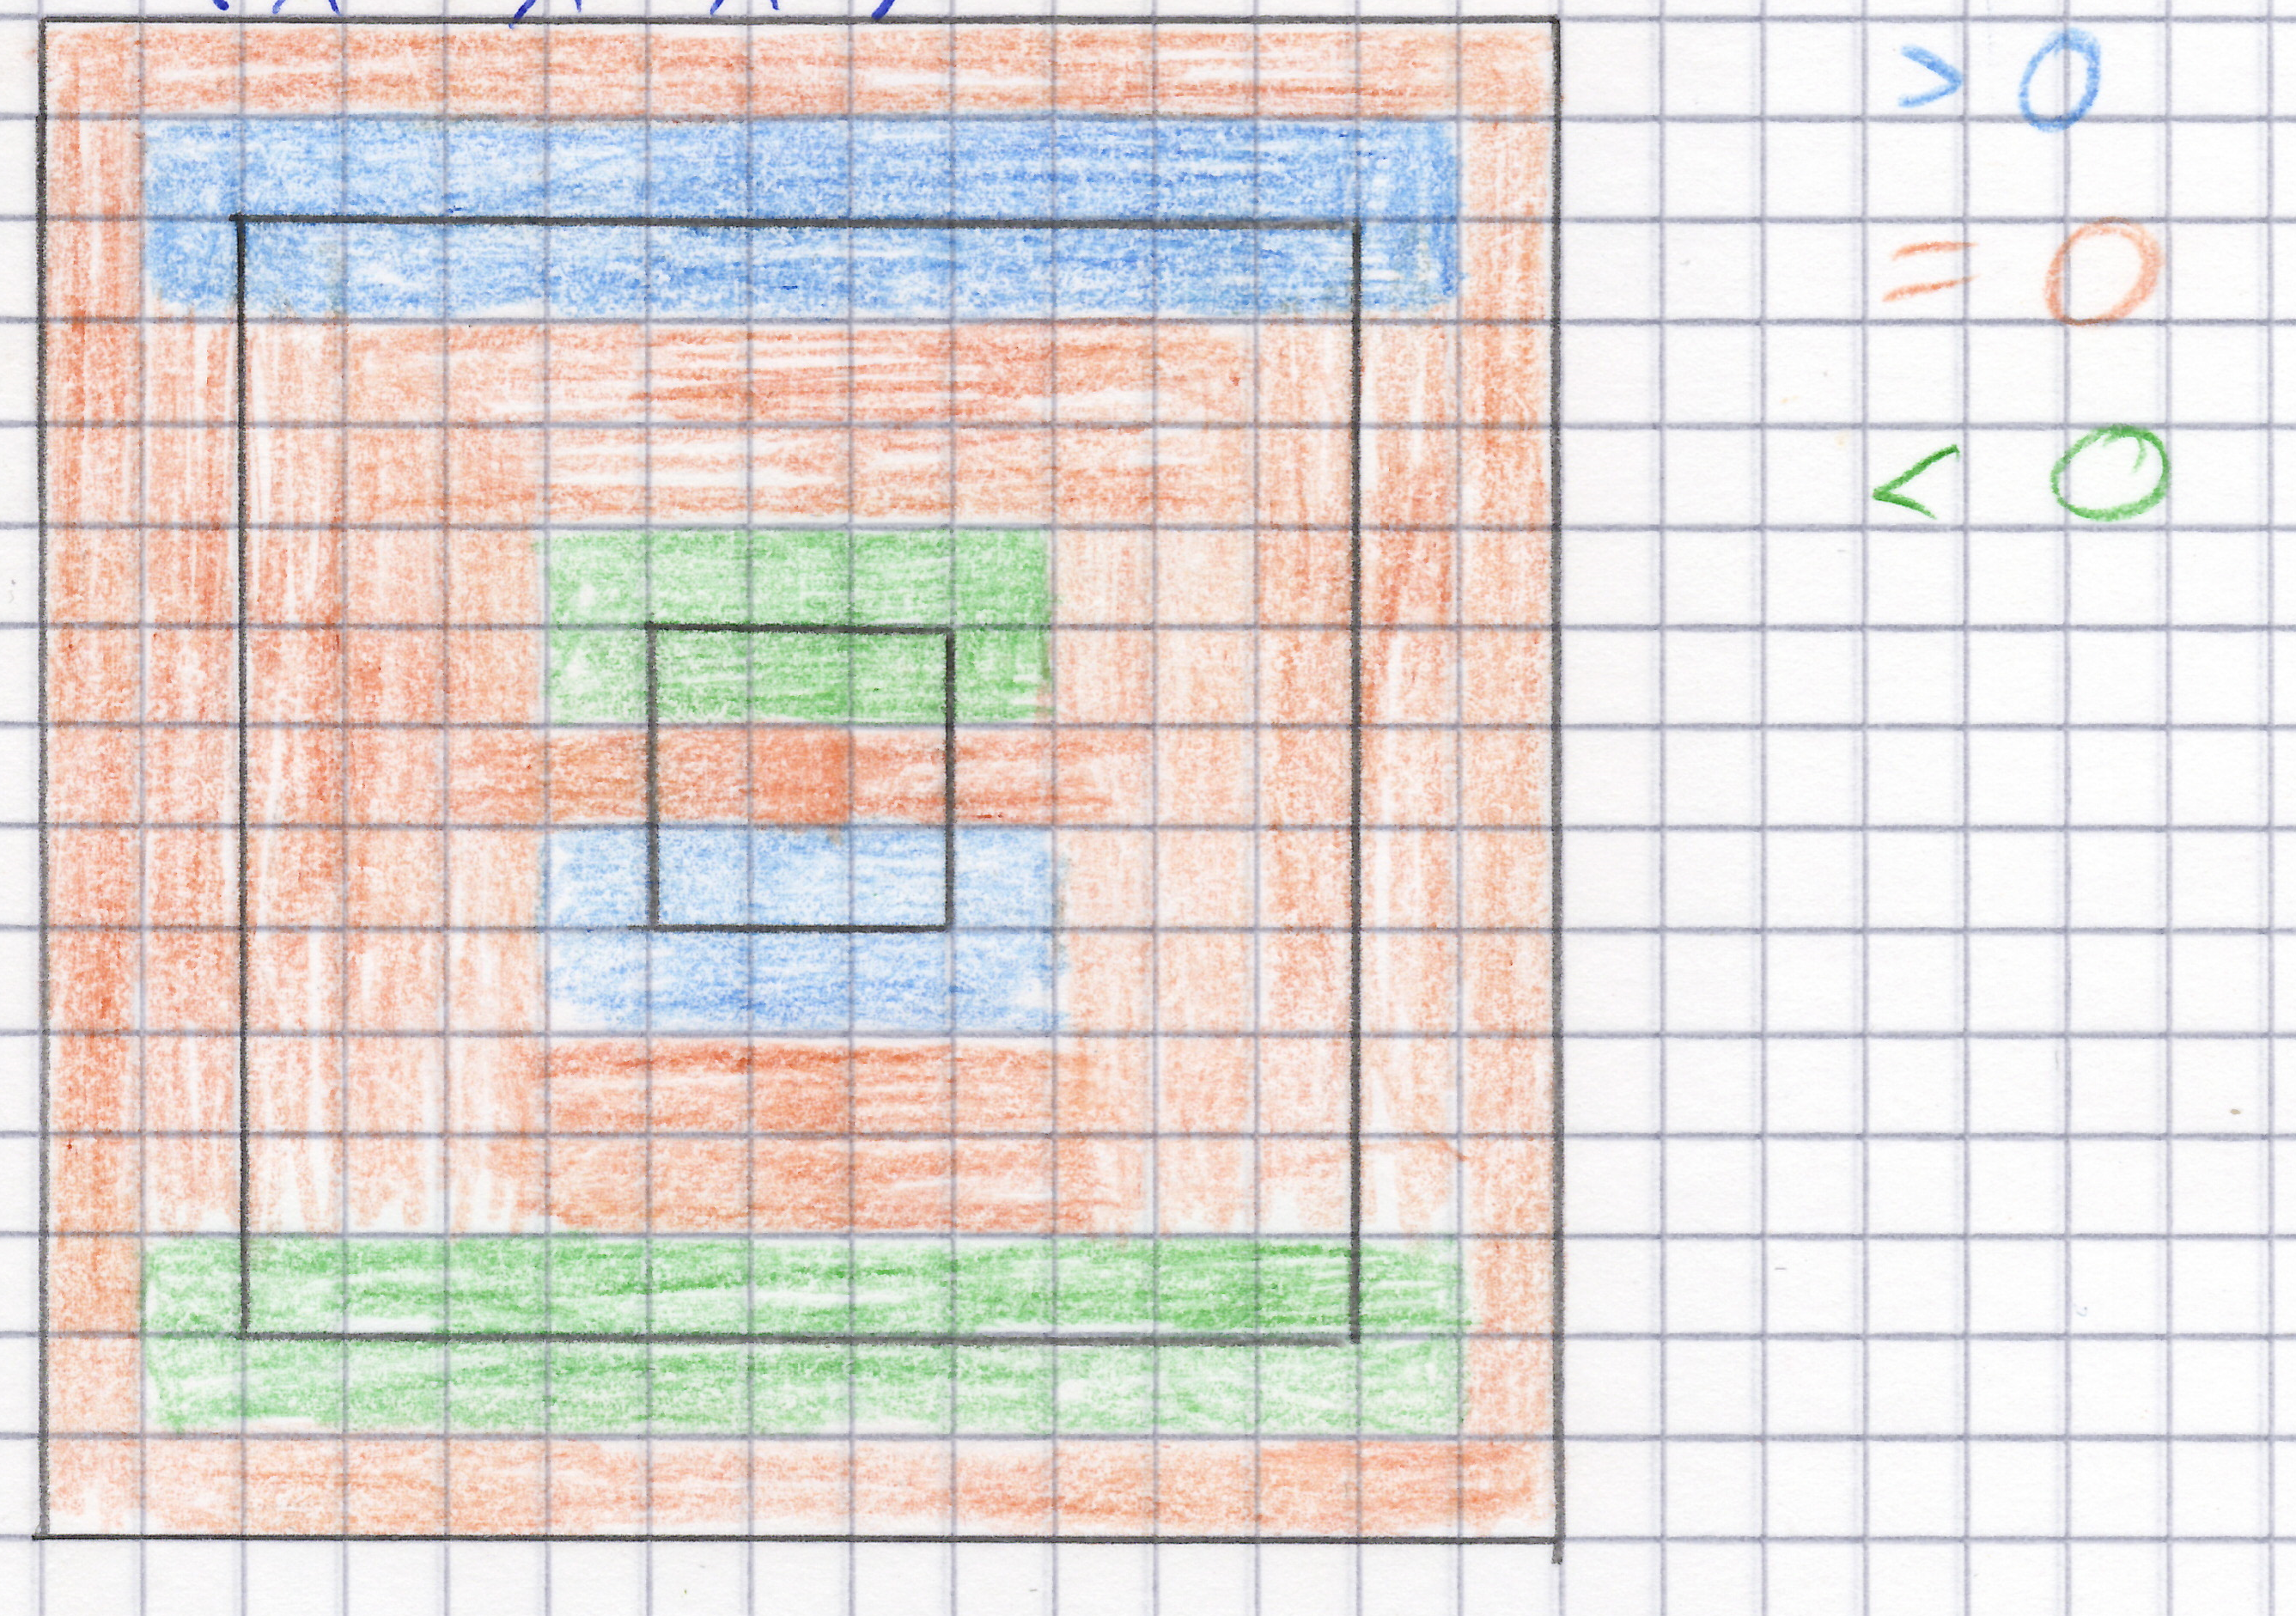
\includegraphics[scale=0.25]{GY.png}
		\caption{Response type of $G_y$ applied to the Figure} 
	\end{center}
\end{figure}
\end{document}